% Directly authored PI companion; LaTeX is the editable master.
% Compile from the repository root:
% latexmk -pdf -outdir=/tmp/gamma-scale-pi-latex docs/gamma_scale_acquisition_pi_brief.tex
% Rebuild only the evidence figures:
% MPLCONFIGDIR=/tmp/gamma-pi-mpl .venv/bin/python -m experiments.expD34_readout_race.pi_brief_figures
\documentclass[10pt]{article}
\usepackage[T1]{fontenc}
\usepackage{amsmath,amssymb}
\usepackage{newtxtext,newtxmath}
\usepackage[letterpaper,margin=0.65in]{geometry}
\usepackage{graphicx,microtype,xcolor,caption,fancyhdr,booktabs,tabularx}
\usepackage[colorlinks=true,linkcolor=blue!45!black,urlcolor=blue!55!black]{hyperref}
\definecolor{ink}{HTML}{263442}
\DeclareMathOperator{\sech}{sech}
\DeclareMathOperator{\sign}{sign}
\newcommand{\avg}[1]{\langle #1\rangle_m}
\newcommand{\norm}[1]{\left\|#1\right\|}
\graphicspath{{docs/assets/gamma_scale_acquisition_pi_brief/}{assets/gamma_scale_acquisition_pi_brief/}}
\hypersetup{pdftitle={Why joint training may fail to acquire useful scales},
  pdfsubject={Readout-geometry competition: empirical evidence, early depletion, and effective slope sensitivity}}
\setlength{\parindent}{0pt}
\setlength{\parskip}{5pt plus 1pt}
\setlength{\emergencystretch}{2em}
\setlength{\headheight}{13pt}
\captionsetup{font=small,labelfont=bf,justification=raggedright,singlelinecheck=false}
\pagestyle{fancy}
\fancyhf{}
\fancyhead[L]{\small\color{ink}Readout--geometry competition}
\fancyhead[R]{\small PI research brief}
\fancyfoot[C]{\small\thepage}
\renewcommand{\headrulewidth}{0.3pt}

\begin{document}
\thispagestyle{plain}
{\color{ink}\fontsize{22}{25}\selectfont\bfseries Why joint training may fail\\to acquire useful scales\par}
\vspace{3pt}
\textbf{Readout learning changes the residual that drives slope learning.}
The companion brief, \emph{Gamma controls readout learning speed}, establishes
why scale matters. Here we ask why joint training often fails to acquire it.
Rate interventions support competition between readout and geometry; an early
theorem captures signal depletion; the current approach asks which remaining
errors can still drive slope growth. GD and Adam help separate gradient activity
from sustained outward motion. A quantitative long-time prediction is still open.

{\small
\textbf{Notation.} Parameter-vector norms are Euclidean; residual norms use the stated data measure.\par
\begin{tabularx}{\linewidth}{@{}lX@{}}
\toprule
$a_j,b_j,w_j,d$ & Hidden slope, hidden bias, readout weight, and output bias.\\
$\gamma_j=|a_j|$, $\bar\gamma$ & Individual slope magnitude and its population mean.\\
$r=f-y$, $L=\|r\|_m^2/2$ & Residual and half-MSE; $\|r\|_m^2=m^{-1}\sum_i r(x_i)^2$.\\
$\kappa$, $t=\eta n$ & Readout/geometry rate ratio and flow clock for GD update $n$.\\
$e_C,e_H$, $\mu_a^{\rm eff}$ & Mean/linear error, remaining error, and effective slope sensitivity (Section 3).\\
\bottomrule
\end{tabularx}}

\section*{1. Empirical motivation: changing the race changes gamma}
The jointly trained model is
\begin{equation}\label{eq:model}
 f(x)=d+\sum_{j=1}^W w_j\tanh(a_jx+b_j).
\end{equation}
Our first mechanistic evidence was that reparameterizing readout versus
geometry changed gamma acquisition. A fixed scaling
$\theta=Du$ makes a GD step in $u$ induce
$\Delta\theta=-\eta DD^T\nabla_\theta L$. For example, training signed slopes
in grid units $h a_j$, with fixed reference spacing $h$, multiplies the physical
slope step by $h^{-2}$.
These changes alter the relative mobility of readout and geometry.
The subsequent direct intervention isolates the rate ratio: keep slope and
hidden-bias rate $\eta$ fixed, and vary the readout and output-bias rate
$\kappa\eta$, from exactly the same random initial parameters [1].

\textbf{Why measure the mean and linear trend?}
At small initialization, $\tanh(a_jx+b_j)\approx a_jx+b_j$, so the network
mainly represents a constant plus a linear trend. We call the projection of
the residual onto these two functions the \emph{coarse error}; the remaining
non-affine error is the \emph{fine error}. This is a definition of what we
measure, not an assumption that training has already fitted it.
Figure~\ref{fig:rates} tests whether faster readout fitting leaves less slope
growth. Each horizontal position is a different rate ratio, not a training time.

\begin{figure}[h!]
 \centering
 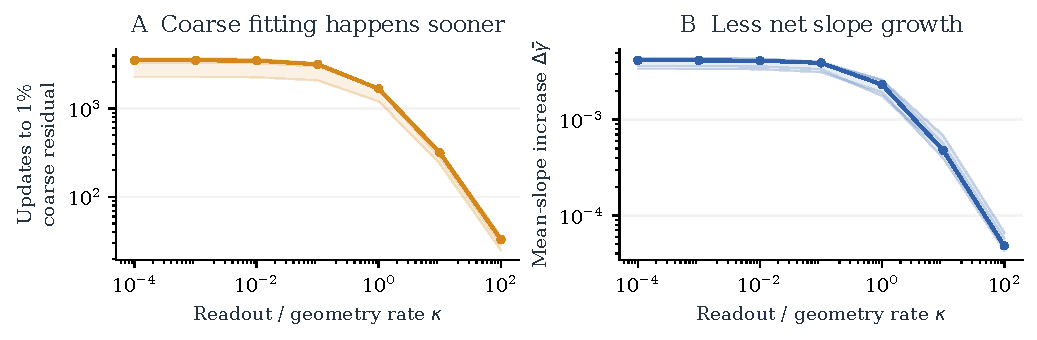
\includegraphics[width=\linewidth]{rate_intervention.pdf}
 \caption{\textbf{Faster readout fits the mean and linear trend sooner, while gamma grows less.}
 A: updates until the coarse-error norm reaches 1\% of its initial value.
 B: net change in mean $\gamma$ after the same 20,000 updates.
 The illustrative target combines a constant, a linear trend, and a degree-nine
 polynomial component. All parameters train simultaneously: $W=177$,
 2,048 training points, geometry rate $0.002$, five paired seeds.
 Bold lines are medians; faint lines and shading show the seeds.}
 \label{fig:rates}
\end{figure}

The trend is consistent with a race: readout adaptation can reduce the error
that would otherwise move the slopes, before much gamma growth accumulates.
Fine error remains large, and the growth contrast is also present when runs
are compared at the same coarse-error threshold. This is mechanistic evidence
for competition. Its direction varies with the target, so it does not yet
give a universal rule for choosing the relative rates.

\clearpage
\section*{2. First proof idea: quantify early signal depletion}
The first proof asks whether readout fitting removes an initially available
slope signal while appreciable error remains. A small gradient alone does not
answer this: it might simply reflect successful fitting. We therefore study
\begin{equation}\label{eq:xi}
 R(t)=\|r(t)\|,\qquad g_a=\nabla_aL,\qquad
 \Xi(t)=\frac{\|g_a(t)\|}{R(t)}.
\end{equation}
This is the current slope gradient per unit residual, including any signal
regenerated during training [2].

\textbf{The theorem's setting.}
Use equal-rate gradient flow, continuous $L^2(dx/2)$ loss on $[-1,1]$,
no output bias, and \emph{zero initial readout}.
Hidden slopes and biases are independent uniforms on
$[-\sqrt{6/(W+1)},\sqrt{6/(W+1)}]$.
The fixed target $y$ is centered, normalized, and entire, with
$\beta=3\langle y,x\rangle\ne0$ and $\|y-\beta x\|>0$.
For each fixed $H_0>3$, at sufficiently large width and with arbitrarily high
fixed probability, signal first forms at a width-independent time $t_f$,
then obeys
\begin{equation}\label{eq:depletion}
 \Xi(t_f)\ge s_y>0,\qquad
 \Xi(t)\le C_{y,H_0}\bigl(e^{-t/3}+W^{-1}\bigr),
 \quad 0\le t\le H_0\log W.
\end{equation}
In particular, $\Xi=O(W^{-1})$ throughout
$[3\log W,H_0\log W]$, even though the target has a non-affine component.

\textbf{Why the proof works.}
At small preactivations, tanh is approximately affine. Its exact slope
gradient can be written
\begin{equation}\label{eq:affine-remainder}
 (g_a)_j=w_j\langle r,x\rangle
 -w_j\langle r,x\tanh^2(a_jx+b_j)\rangle.
\end{equation}
The coupled affine reference describes fitting the constant and linear
moments. A parameter comparison and nonlinear remainder estimates bound both
their regeneration and the second term in \eqref{eq:affine-remainder}.
Thus the theorem bounds the total surviving signal, rather than merely
showing that the initial coarse residual disappeared.

\textbf{Where the readout enters.}
Let $q=(a,b)$ and let $\mathsf H_{aI}$ be the corresponding loss-Hessian block.
Where $\|g_a\|,R>0$, equal-rate flow gives the exact identity
\begin{equation}\label{eq:attribution}
 -\frac{d}{dt}\log\Xi=D_w+D_q,\qquad
 D_I=\frac{g_a^T\mathsf H_{aI}g_I}{\|g_a\|^2}
       -\frac{\|g_I\|^2}{R^2}.
\end{equation}
On the shorter attribution window from $t_f$ to
$t_f+\rho\log W/\nu_y$, with $0<\rho<1/2$ and
$\nu_y=2\sqrt{1+\beta^2}/3$, the readout's share
of the leading logarithmic decline tends in probability to
\begin{equation}\label{eq:share}
 \pi_y=\frac12+\frac{1}{2\sqrt{1+\beta^2}}\in(3/4,1).
\end{equation}
This is a signed attribution along the joint trajectory. It says more than
three quarters of that leading decline is attributable to readout adaptation;
it is not three quarters of all possible gamma growth, or a frozen-readout
counterfactual. Individual contributions can later become negative.

\textbf{Why this was not yet quantitatively predictive.}
The proof supplies width and time scaling, but its conservative constants do
not give tight bounds at our experimental widths. Uniform remainder estimates
can be much larger than the surviving signal they bound. The asymptotic
readout share quantifies a mechanism, but does not predict how far gamma moves,
when useful scales are reached, or whether nonlinear forcing later recovers.
The guarantee also covers an early logarithmic-time window and a zero-readout
law, whereas the long D34 trajectories start with random nonzero readouts.
Accurate cubic or quintic reference forecasts help, but measured agreement
does not certify a uniformly small error envelope.

The proof establishes an early mechanism. The next task is to explain the
force that remains, including its subsequent recovery, on the actual training
trajectory. That motivates resolving the gradient-flow equations more directly.

\clearpage
\section*{3. Current approach: identify the force that still moves slopes}
Return to the empirical model \eqref{eq:model}, with all four blocks trained,
random nonzero readouts, and equal physical rates. Its slope equation is
\begin{equation}\label{eq:slope}
 \dot a_j=-(g_a)_j
 =-w_j\avg{r(x)\,x\,\sech^2(a_jx+b_j)}.
\end{equation}
Residual size alone cannot determine this velocity: the residual must align
with each current slope tangent, and the readout weight multiplies that tangent.
We now separate the contribution associated with the mean and linear trend
from the force supplied by the remaining error [3].

\textbf{Resolve the residual into coarse and fine components.}
Choose a fixed empirical orthonormal basis $q_k(x)$ on the training points,
with $q_0=1$, $q_1=x/\sqrt{\avg{x^2}}$ on the symmetric grid.
Set $e_k=\avg{q_k r}$, $e_C=(e_0,e_1)^T$, and let $e_H$ contain the
\emph{complete} remaining complement. Define the modal Jacobian block
$(J_I)_{kj}=\avg{q_k\,\partial f/\partial\theta_{I,j}}$ for
$I\in\{a,b,w,d\}$. Then $g_I=J_I^Te$, and equal-rate flow gives
\begin{equation}\label{eq:modal}
 \dot e=-Ke,\qquad K=\sum_I J_IJ_I^T,
 \qquad
 \begin{aligned}
 \dot e_C&=-K_{CC}e_C-K_{CH}e_H,\\
 \dot e_H&=-K_{HC}e_C-K_{HH}e_H.
 \end{aligned}
\end{equation}
All parameter blocks contribute to $K$. The coarse/fine split concerns output
error, rather than a split between readout and geometry parameters.

\textbf{Coarse equilibrium is generally nonzero.}
If $K_{CC}$ is invertible, hold its current blocks and $e_H$ fixed to find
the instantaneous coarse balance:
\begin{equation}\label{eq:balance}
 B=K_{CC}^{-1}K_{CH},\qquad
 e_C^{\rm bal}=-Be_H,\qquad z_C=e_C+Be_H.
\end{equation}
Here $z_C$ measures disagreement with that moving balance. Substituting
$e_C=-Be_H+z_C$ into the slope gradient and fine-residual equation gives
\begin{equation}\label{eq:effective}
 \boxed{\ g_a=J_{a,C}^Tz_C+T_ae_H,\qquad
          \dot e_H=-Se_H-K_{HC}z_C\ },
\end{equation}
\begin{equation}\label{eq:maps}
 T_a=J_{a,H}^T-J_{a,C}^TB,\qquad
 S=K_{HH}-K_{HC}B.
\end{equation}
The first force in \eqref{eq:effective} comes from imperfect tracking;
the second survives at coarse balance. Crucially, $T_ae_H$ includes the
balanced coarse response $-J_{a,C}^TBe_H$. Setting $e_C=0$ would omit it.
``Fine'' also includes generated low-degree nonlinear errors, not only the
hardest target mode. These identities are exact for the full complement;
a truncated modal calculation must retain its omitted-residual corrections.

\textbf{Why focus on the effective fine force?}
Across the post-transient GD panel (13 targets, five seeds), $J_{a,C}^Tz_C$
is small and $T_ae_H$ accounts for nearly the whole slope gradient [4]. Adam gives a useful
contrast: coarse disagreement can be large without supplying positive net
gamma growth (Figure~\ref{fig:force}). Thus the quantity to understand is
the surviving force and its sustained outward direction, not residual size
or instantaneous gradient magnitude alone.

\textbf{Arriving at the effective sensitivity.}
For $R_H=\|e_H\|>0$, let $u_H=e_H/R_H$ and define
\begin{equation}\label{eq:sensitivity}
 G_a=T_a^TT_a,\qquad
 \boxed{\ \mu_a^{\rm eff}=u_H^TG_au_H
       =\frac{\|T_ae_H\|^2}{\|e_H\|^2},\qquad
       \|T_ae_H\|=R_H\sqrt{\mu_a^{\rm eff}}\ }.
\end{equation}
This is a squared, direction-dependent sensitivity of slopes to the current
fine residual. It separates \emph{how much error remains} from \emph{how
strongly that error can move the slopes}. It also incorporates interference
between direct fine forcing and the induced coarse response.

\clearpage
{\color{ink}\large\bfseries Large gradient activity need not acquire scale}\par
In the mixed-sine example, coarse disagreement is small in GD but comparable
to the full slope gradient in Adam. Yet it supplies no positive signed
mean-gamma growth in any of the five Adam seeds shown.
\begin{figure}[h!]
 \centering
 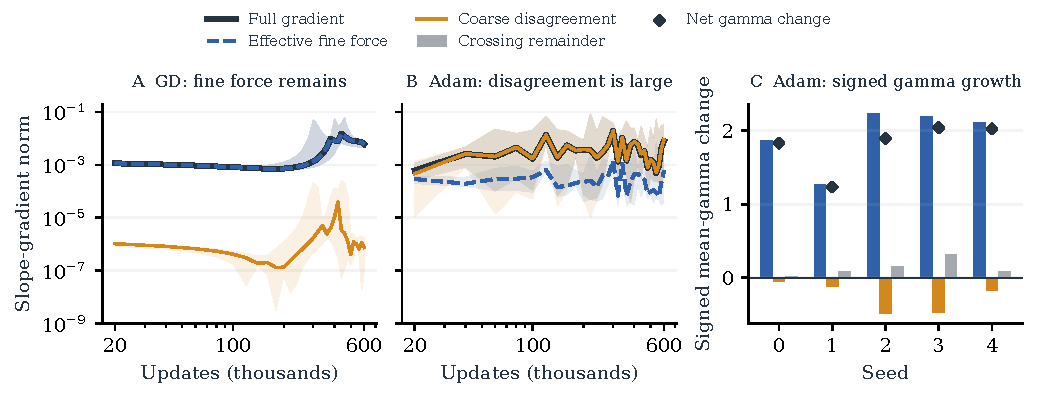
\includegraphics[width=\linewidth]{force_and_motion.pdf}
 \caption{\textbf{Adam's large coarse-disagreement force does not imply outward growth.}
 A--B: gradient norms on each optimizer's trajectory, with a shared vertical
 scale; lines are five-seed medians, shading spans seeds. C: signed Adam
 contributions accumulated at every update; diamonds show net growth and gray
 accounts for zero crossings. Orange is negative despite its large norm in B.
 A normalized sum of three sine waves; $W=177$, 2,048 points, rate $0.002$,
 updates 20,000--600,000 [4].}
 \label{fig:force}
\end{figure}

\textbf{For Adam, the test must use the actual updates.}
Split the first-moment history by channel and apply the \emph{same actual
second-moment denominator} to both. Then
$\Delta a_n=\Delta a_n^{\rm eff}+\Delta a_n^{\rm track}$, with exact accounting
\begin{equation}\label{eq:adam-motion}
 D_k=\sum_n\frac{\sign(a_n)^T\Delta a_n^k}{W},\qquad
 \Delta\bar\gamma=D_{\rm eff}+D_{\rm track}+X.
\end{equation}
Here $X\ge0$ is the absolute-value remainder at zero crossings. Coarse activity
mostly cancels or points inward, while the fine channel supplies positive drift.
Tracking can contribute positively on other targets; this accounting does not
establish what removing it would do. Large disagreement also remains when
the instantaneous balance uses Adam's metric [4].

\textbf{Back in gradient flow, the race has an explicit dynamical form.}
Write $F_a=T_ae_H$. Differentiating the force gives
\begin{equation}\label{eq:force-evolution}
 \dot F_a=
 \underbrace{\dot T_ae_H}_{\text{changing sensitivity map}}
 -\underbrace{T_aSe_H}_{\text{evolving fine residual}}
 -\underbrace{T_aK_{HC}z_C}_{\text{tracking correction}}.
\end{equation}
Readout evolution changes both $T_a$ and $S$: coupling can improve while the
driving residual depletes or rotates. Both weakening and renewed forcing
remain possible.

To connect sensitivity to acquisition, define the signed outward alignment
$\chi_a=-\sign(a)^TF_a/(\sqrt W\|F_a\|)$ where $F_a\ne0$.
Away from slope zero crossings, the exact flow identity is
\begin{equation}\label{eq:outward}
 \dot{\bar\gamma}
 =\frac{R_H\sqrt{\mu_a^{\rm eff}}\,\chi_a}{\sqrt W}
  -\frac{\sign(a)^TJ_{a,C}^Tz_C}{W},\qquad |\chi_a|\le1.
\end{equation}
Sensitivity measures available force; alignment determines outward growth.
A population claim also needs its distribution across neurons. Adam requires
the filtered, preconditioned direction in \eqref{eq:adam-motion}.

\textbf{Working hypothesis.}
Readout--geometry feedback may weaken sensitivity or deplete useful residual
directions before enough outward motion accumulates. Controlling
$R_H\sqrt{\mu_a^{\rm eff}}$ and its alignment could predict acquisition time
or bound attainable motion. This connects the ODEs directly to gamma growth;
the missing proof is control of that feedback over time.

\vspace{2pt}
{\footnotesize
\textbf{Sources and reproduction.}
\href{run:../results/checkpoint_D_optimizers/expD34_readout_race/REPORT.md}{[1] D34 rate intervention};
\href{run:readout_driven_slope_signal_depletion.md}{[2] Early-depletion theory, 20 September 2026};
\href{run:d34_transport_scale_barrier.md}{[3] Coupled-force theory};
\href{run:../results/checkpoint_D_optimizers/expD34_readout_race/adam_force_extension/README.md}{[4] Expanded GD/Adam force study}.
The companion motivation is
\href{run:../../precision-mlps-frozen-gamma-probe/docs/gamma_optimization_pi_brief.pdf}{\emph{Gamma controls readout learning speed}}.
Figures replot existing fp64 runs. Inputs, values, checks, and hashes are in
\href{run:assets/gamma_scale_acquisition_pi_brief/evidence.json}{the evidence record}.
Figure and PDF rebuild commands are in the LaTeX source. Links resolve locally.
}
\end{document}
